\section{Dataset}
In this section we briefly describe the dataset on which we tested some of the previously presented algorithms. The dataset used is the NASDAQ-2196\footnotemark[1]; this dataset is a $2196 \times 2196$ covariance matrix with:\footnotetext[1]{NASDAQ-2196 dataset can be downloaded at \url{http://host.uniroma3.it/docenti/cesarone/datasetsw3_tardella.html}}
\begin{itemize}
\item $\min \{\Sigma_{\text{NQ}}\} = -7.5347 \times 10^{-3} $
\item $\max \{\Sigma_{\text{NQ}}\} = 6.0531 \times 10^{-2} $
\item $\mu(\Sigma_{\text{NQ}}) = 4.1252 \times 10^{-4} $
\item $\sigma^2(\Sigma_{\text{NQ}}) = 2.9305 \times 10^{-7}$
\end{itemize}
In all the following experiments we used the NASDAQ-2196 dataset; from the covariance matrix contained in the dataset, we compute the correlation matrix and we use that instead of the covariance one for numerical reasons.

\section{Implementation details}
All the algorithms are written in \textit{Python 2.7} while we use the official Python interface for SNOPT. We also use \texttt{numpy} library, linked with \texttt{blas} and \texttt{ATLAS} libraries. The PC used for the experiments is equipped with and Intel i7 3630QM processor, 8GB of RAM and a Linux based distribution. We use \texttt{time.clock()} to determine the execution time of an algorithm, in this way:\\
\texttt{init = time.clock()}\\
\texttt{..execute algorithm..}\\
\texttt{exetime = time.clock() - init}

\section{Convex formulation}
In this section we compare the execution time of two algorithms used to solve the convex RP Problem (\ref{eq:log1}): CCD and Newton-Nesterov.
\subsection{Test problems and stopping criterion}
We use the same stop criterion for both the algorithms tested; we stop the algorithm when:
\begin{equation}\label{eq:stopconv}
\max_i \left| \frac{RC_i}{\mathcal{R}(x)} - \frac{1}{n} \right| < \eta
\end{equation}
Equation (\ref{eq:stopconv}) express the fact that the (normalized) max deviation from Risk Parity of the solutions is less than $\eta$.
\begin{figure}
\centering
\makebox[\textwidth][c]{
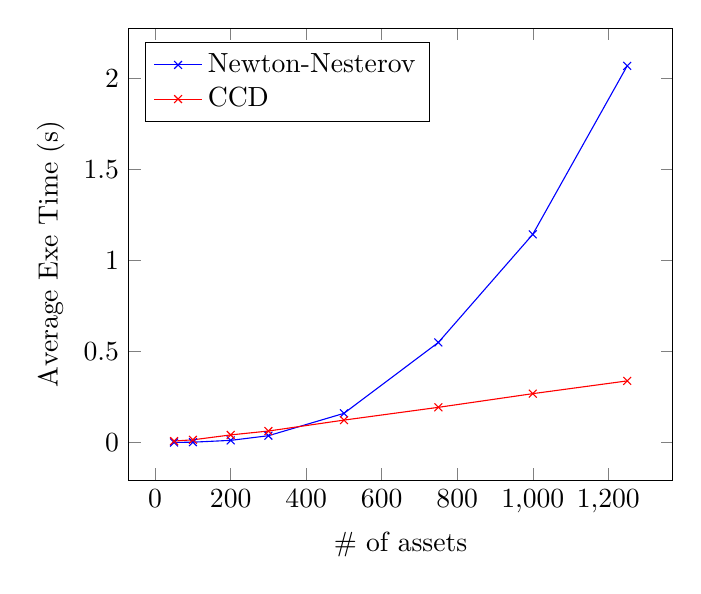
\begin{tikzpicture}

\begin{axis}[%
width=0.7\textwidth,
xlabel={\# of assets},
ylabel={Average Exe Time (s)},
legend pos=north west,
legend cell align=left
]
\addplot [color=blue,solid,mark=x,mark options={solid}]
  table[row sep=crcr]{%
50	.0013		\\
100	.0029	\\
200 .0128		\\
300 .0383        \\
500	.161		\\
750	.550		\\
1000 1.143		\\
1250	 2.067	\\
};

\addplot [color=red,solid,mark=x,mark options={solid}]
  table[row sep=crcr]{%
50	.009	\\
100	.0158		\\
200	.0427		\\
300 .064        \\
500	.124		\\
750	.194		\\
1000	 .269\\
1250	 .339	\\
};
\addlegendentry{Newton-Nesterov}
\addlegendentry{CCD}
\end{axis}
\end{tikzpicture}
}
\caption{Comparison of average execution time between CCD and Newton-Nesterov with $\eta = 10^{-8}$ in the stop criterion (\ref{eq:stopconv})}
\label{fig:convtest}
\end{figure}
Figure (\ref{fig:convtest})  shows that, for an universe of a small number of assets ($n<200$), Newton-Nesterov algorithm performs better than CCD. On the other hand, when we consider a bigger asset's universe ($n>300$), CCD outperform Newton-Nesterov; with $n=1250$, CCD algorithm is approximately 8 times faster to converge than the Newton-Nesterov one.
\section{Least-square formulation}
In this section we compare the decomposition algorithm against SNOPT \cite{snopt}.

\subsection{Test problems and stopping criterion}
In order to obtain comparable results, in our scheme we use a stop criterion that is the same used by SNOPT, i.e. we stop the algorithm when
\begin{equation}\label{eq:stop}
\left| \frac{\partial f(x^k,y^k)}{d{x_{j(k)}}} - \frac{\partial f(x^k,y^k)}{d{x_{i(k)}} }\right| < \epsilon
\end{equation}
In SNOPT, this is (almost) equivalent to set the\linebreak \texttt{Major optimality tolerance} optional parameter to $\epsilon$.\\
In the following experiments, we denote with DEC$_{\text{MVP}}$ Algorithm \ref{alg:proximal} with $M=1$ (we compute the MVP among the full gradient $\nabla_x f(x,y)$ at each iteration), while we denote with DEC$_{\text{MVP-}\lambda\%}$ Algorithm \ref{alg:modified}. For DEC$_{\text{MVP-}\lambda\%}$ we evaluate the stop criterion (\ref{eq:stop}) every $M$ iterations (when we have the full gradient available).

\subsection{Classical box constraints}
In this section we use 
\begin{equation}\label{eq:classicalbox}
l_i = 0  \qquad u_i = 1  \quad \forall i
\end{equation} 
\subsubsection{Inexact vs Exact Line Search}
In Figure (\ref{fig:els}) we compare the performances of the decomposition algorithm using two different step selection: Algoritm \ref{alg:decMVP}, that uses Quadratic Line Search (QLS) and Algorithm \ref{alg:proximal} that uses Exact Line Search (ELS) instead, using the following starting point:
\begin{equation}\label{eq:sparsestarting}
x^0 = \left[1, 0, .., 0 \right]
\end{equation}
Figure (\ref{fig:els}) points out that Algorithm \ref{alg:proximal} performs better than Algorithm \ref{alg:decMVP} in this particular problem. From now on, we always use the Proximal Point version of the decomposition algorithm (Algorithm \ref{alg:proximal}) in the next experiments.

\begin{figure}
\makebox[\textwidth][c]{
\subfloat[Comparison of average execution time\label{subfig-4:time2}]{%
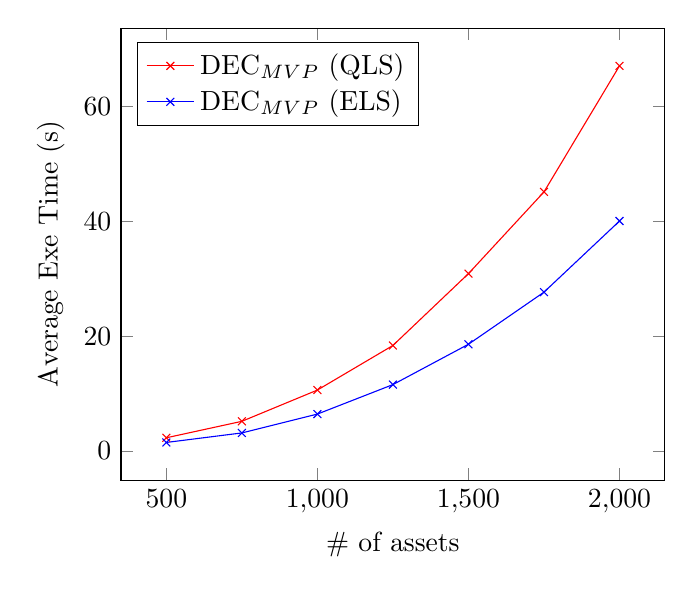
\begin{tikzpicture}
\begin{axis}[%
width=0.7\textwidth,
xlabel={\# of assets},
ylabel={Average Exe Time (s)},
scaled y ticks=false,
legend pos=north west,
legend cell align=left
]

\addplot [color=red,solid,mark=x,mark options={solid}]
  table[row sep=crcr]{%10
500 2.30\\
750 5.17\\
1000 10.62\\
1250 18.39\\
1500 30.91\\
1750 45.15\\
2000 67.12\\
};

\addplot [color=blue,solid,mark=x,mark options={solid}]
  table[row sep=crcr]{%5
500	1.486	\\
750	3.147	\\
1000 6.431 \\
1250 11.57 \\
1500 18.6  \\
1750 27.68 \\
2000 40.08\\
};

\addlegendentry{DEC$_{\text{MVP}}$ (QLS)}
\addlegendentry{DEC$_{\text{MVP}}$ (ELS)}
\end{axis}

\end{tikzpicture}
}
}
\makebox[\textwidth][c]{
\subfloat[Comparison of average iterations\label{subfig-4:iterations2}]{%
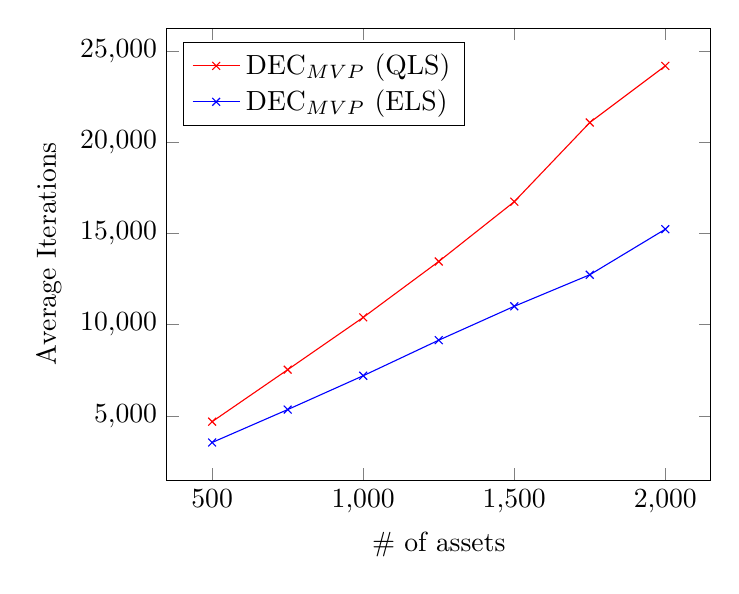
\begin{tikzpicture}

\begin{axis}[%
width=0.7\textwidth,
xlabel={\# of assets},
ylabel={Average Iterations},
scaled y ticks=false,
legend pos=north west,
legend cell align=left
]

\addplot [color=red,solid,mark=x,mark options={solid}]
  table[row sep=crcr]{%10
500 4680 \\
750 7532 \\
1000 10401\\
1250 13469\\
1500 16750\\
1750 21095\\
2000 24204\\
};

\addplot [color=blue,solid,mark=x,mark options={solid}]
  table[row sep=crcr]{%5
500	 3538\\
750	 5343 \\
1000	  7200\\
1250 9151\\
1500 11011\\
1750 12741\\
2000 15241\\
};

\addlegendentry{DEC$_{\text{MVP}}$ (QLS)}
\addlegendentry{DEC$_{\text{MVP}}$ (ELS)}
\end{axis}

\end{tikzpicture}
}
}
\caption{Comparison of performances using $\epsilon = 10^{-10}$ in (\ref{eq:stop}) with box constraints defined in (\ref{eq:classicalbox}) between the decomposition algorithm with two different step selection (Quadratic Line Search and Exact Line Search)}
\label{fig:els}
\end{figure}

\subsubsection{Decomposition vs SNOPT}
In Figure (\ref{fig:100}) and Figure (\ref{fig:10}) we compare the average execution time and the average number of iterations performed by the decomposition algorithm (with different values of $\lambda$) against SNOPT using the starting point defined in (\ref{eq:sparsestarting}). The $\epsilon$ in the stop criterion (\ref{eq:stop}) is set to $10^{-10}$. In Figure (\ref{fig:100}) we set $M=100$, while in Figure (\ref{fig:10}) we set $M=10$.\\ The two figures show that SNOPT perform better than DEC$_{MVP}$, but show also that DEC$_{\text{MVP-}\lambda\%}$, especially for low values of $\lambda$, outperforms SNOPT in terms of average execution time when the number of assets $n$ becomes high. As we can see comparing Figure (\ref{fig:100}) with Figure (\ref{fig:10}), parameter $M$ does not significantly affect the performances of the decomposition algorithm, thus we can set $M=100$ in the next experiments.
\begin{figure}
\makebox[\textwidth][c]{
\subfloat[Comparison of average execution time\label{subfig-1:time2}]{%
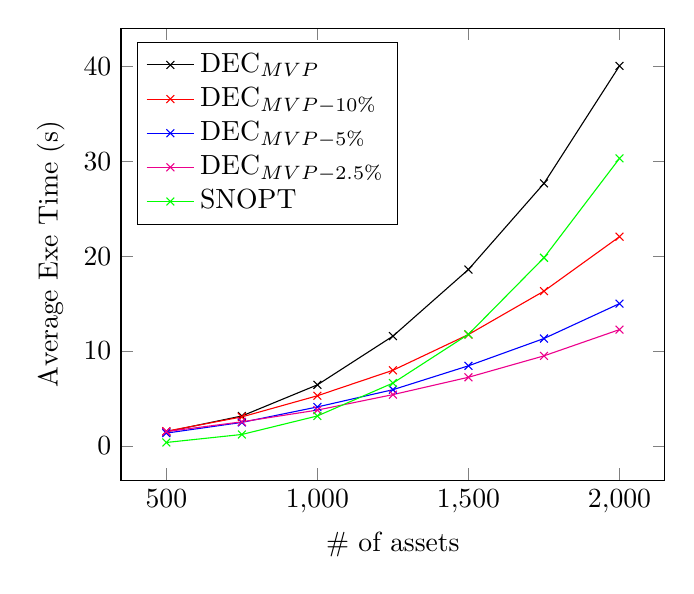
\begin{tikzpicture}
\begin{axis}[%
width=0.7\textwidth,
xlabel={\# of assets},
ylabel={Average Exe Time (s)},
scaled y ticks=false,
legend pos=north west,
legend cell align=left
]

\addplot [color=black,solid,mark=x,mark options={solid}]
  table[row sep=crcr]{%MVP
500	1.486	\\
750	3.147	\\
1000 6.431 \\
1250 11.57 \\
1500 18.6  \\
1750 27.68 \\
2000 40.08\\
};

\addplot [color=red,solid,mark=x,mark options={solid}]
  table[row sep=crcr]{%10
500 1.54\\
750 3.05\\
1000 5.28 \\
1250 7.97\\
1500 11.74\\
1750 16.32\\
2000 22.06\\
};

\addplot [color=blue,solid,mark=x,mark options={solid}]
  table[row sep=crcr]{%5
500 1.34 \\
750 2.47 \\
1000 4.10 \\
1250 5.92\\
1500 8.44 \\
1750 11.32 \\
2000 15.00 \\
};

\addplot [color=magenta,solid,mark=x,mark options={solid}]
  table[row sep=crcr]{%2.5
500  1.50\\
750  2.53\\
1000 3.77 \\
1250 5.40 \\
1500 7.23 \\
1750 9.49 \\
2000 12.26\\
};

\addplot [color=green,solid,mark=x,mark options={solid}]
  table[row sep=crcr]$}
\addlegendentry{DEC$_{\text{MVP-}5\%}$}
\addlegendentry{DEC$_{\text{MVP-}2.5\%}$}
\addlegendentry{SNOPT}
\end{axis}

\end{tikzpicture}
}
}
\hfill
\hspace{1em}\subfloat[Comparison of average iterations\label{subfig-2:iterations2}]{%
\makebox[\textwidth][c]{
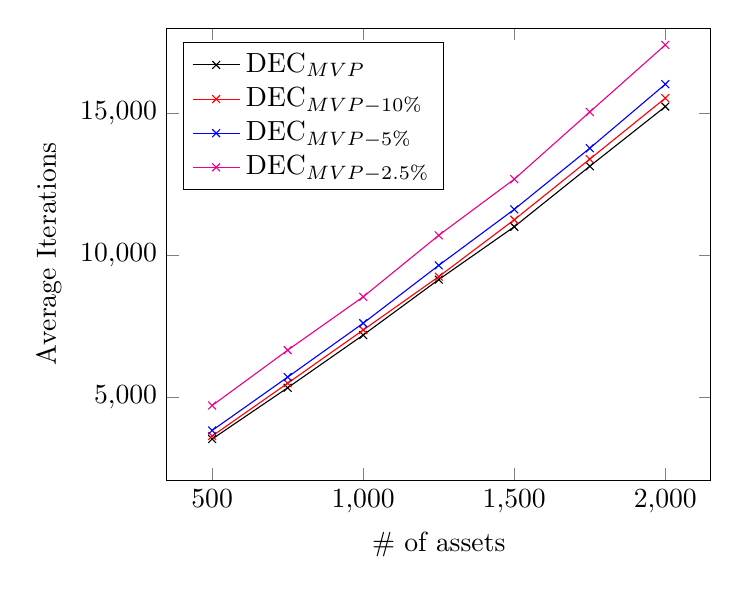
\begin{tikzpicture}

\begin{axis}[%
width=0.7\textwidth,
xlabel={\# of assets},
ylabel={Average Iterations},
scaled y ticks=false,
ymax=18000,
legend pos=north west,
legend cell align=left
]

\addplot [color=black,solid,mark=x,mark options={solid}]
  table[row sep=crcr]{%MVP
500	 3538\\
750	 5343 \\
1000	  7200\\
1250 	9151\\
1500    11011\\
1750 13141\\
2000 15241\\
};

\addplot [color=red,solid,mark=x,mark options={solid}]
  table[row sep=crcr]{%10
500 3644  \\
750 5503 \\
1000 7377 \\
1250 9255 \\
1500 11257 \\
1750 13392 \\
2000 15540\\
};

\addplot [color=blue,solid,mark=x,mark options={solid}]
  table[row sep=crcr]{%5
500 3840   \\
750 5719 \\
1000 7616  \\
1250 9652 \\
1500 11624 \\
1750 13776\\
2000 16029 \\
};

\addplot [color=magenta,solid,mark=x,mark options={solid}]
  table[row sep=crcr]$}
\addlegendentry{DEC$_{\text{MVP-}5\%}$}
\addlegendentry{DEC$_{\text{MVP-}2.5\%}$}
\end{axis}

\end{tikzpicture}
}
}
\caption{Comparison of performances using $\epsilon = 10^{-10}$ in (\ref{eq:stop}) with box constraints defined in (\ref{eq:classicalbox}) with $M=100$}
\label{fig:100}
\end{figure}

\begin{figure}
\centering
\makebox[\textwidth][c]{
\subfloat[Comparison of average execution time\label{subfig-1:time3}]{%
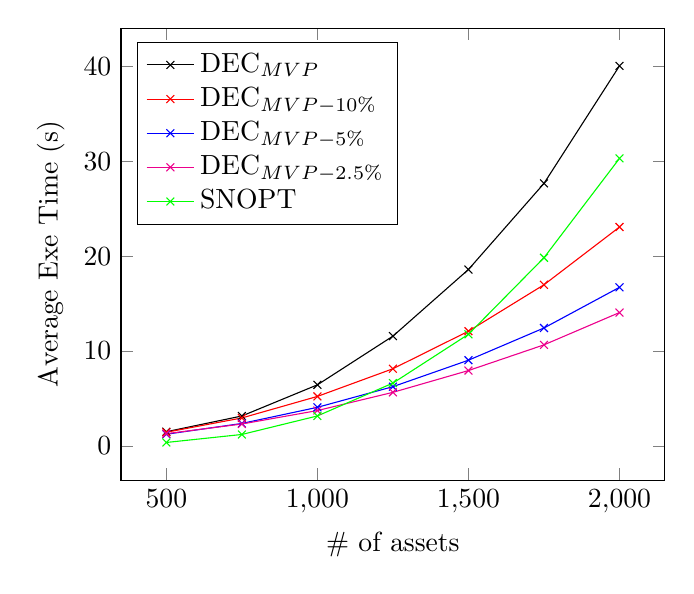
\begin{tikzpicture}
\begin{axis}[%
width=0.7\textwidth,
xlabel={\# of assets},
ylabel={Average Exe Time (s)},
scaled y ticks=false,
legend pos=north west,
legend cell align=left
]

\addplot [color=black,solid,mark=x,mark options={solid}]
  table[row sep=crcr]{%MVP
500	1.486	\\
750	3.147	\\
1000 6.431 \\
1250 11.57 \\
1500 18.6  \\
1750 27.68 \\
2000 40.08\\
};

\addplot [color=red,solid,mark=x,mark options={solid}]
  table[row sep=crcr]{%10
500 1.43\\
750 2.94\\
1000 5.21 \\
1250 8.13\\
1500 12.09\\
1750 16.99\\
2000 23.08\\
};

\addplot [color=blue,solid,mark=x,mark options={solid}]
  table[row sep=crcr]{%5
500 1.22 \\
750 2.36 \\
1000 4.06 \\
1250 6.24\\
1500 9.03 \\
1750 12.43 \\
2000 16.72 \\
};

\addplot [color=magenta,solid,mark=x,mark options={solid}]
  table[row sep=crcr]{%2.5
500  1.28\\
750  2.30\\
1000 3.72 \\
1250 5.64 \\
1500 7.94 \\
1750 10.65 \\
2000 14.06\\
};

\addplot [color=green,solid,mark=x,mark options={solid}]
  table[row sep=crcr]$}
\addlegendentry{DEC$_{\text{MVP-}5\%}$}
\addlegendentry{DEC$_{\text{MVP-}2.5\%}$}
\addlegendentry{SNOPT}
\end{axis}

\end{tikzpicture}
}
}
\hfill
\hspace{1em}\subfloat[Comparison of average iterations\label{subfig-2:iterations3}]{%
\makebox[\textwidth][c]{
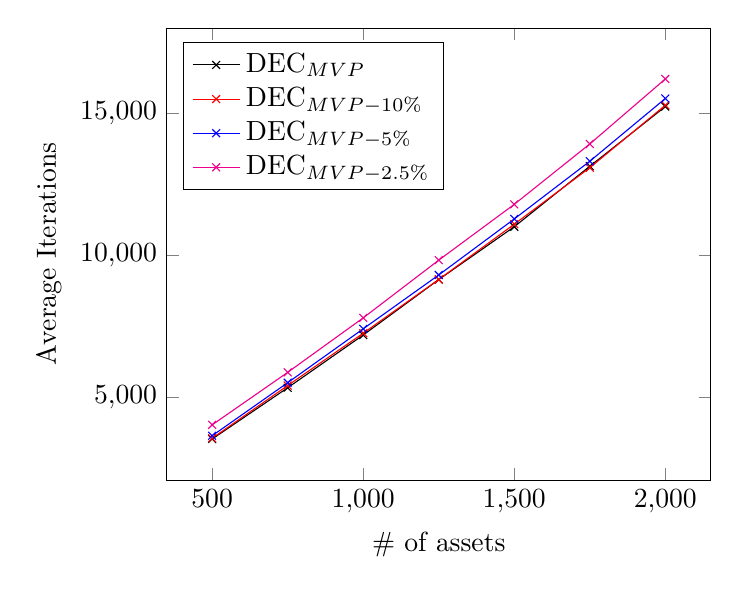
\begin{tikzpicture}

\begin{axis}[%
width=0.7\textwidth,
xlabel={\# of assets},
ylabel={Average Iterations},
scaled y ticks=false,
legend pos=north west,
legend cell align=left,
ymax=18000
]

\addplot [color=black,solid,mark=x,mark options={solid}]
  table[row sep=crcr]{%MVP
500	 3538\\
750	 5343 \\
1000	  7200\\
1250 	9151\\
1500    11011\\
1750 13141\\
2000 15241\\
};

\addplot [color=red,solid,mark=x,mark options={solid}]
  table[row sep=crcr]{%10
500 3565  \\
750 5422 \\
1000 7263 \\
1250 9155 \\
1500 11101 \\
1750 13089 \\
2000 15289\\
};

\addplot [color=blue,solid,mark=x,mark options={solid}]
  table[row sep=crcr]{%5
500 3654   \\
750 5522 \\
1000 7418  \\
1250 9314 \\
1500 11285 \\
1750 13317\\
2000 15526\\
};

\addplot [color=magenta,solid,mark=x,mark options={solid}]
  table[row sep=crcr]$}
\addlegendentry{DEC$_{\text{MVP-}5\%}$}
\addlegendentry{DEC$_{\text{MVP-}2.5\%}$}
\end{axis}

\end{tikzpicture}
}
}
\caption{Comparison of performances using $\epsilon = 10^{-10}$ in (\ref{eq:stop}) with box constraints defined in (\ref{eq:classicalbox}) with $M=10$}
\label{fig:10}
\end{figure}

\subsubsection{Convergence to a Risk Parity solution}
In this section we evaluate the probability to converge to a critical point $(x^*,y^*)$ that is also a Risk Parity solution, i.e. that satisfies 
\begin{equation}\label{eq:reseps}
\max_i \left| \frac{RC_i}{\mathcal{R}(x^*,y^*)} - \frac{1}{n} \right| < \eta
\end{equation}
where $RC_i$ is the risk contribution of the asset $i$ and ${\mathcal{R}(x^*,y^*)}$ is the total risk of the invested portfolio. Equation (\ref{eq:reseps}) express the fact that the (normalized) max deviation from Risk Parity of the solutions is less than $\eta$. In Figure (\ref{fig:convergence1}) we compare the probability to reach a Risk Parity solution for both the decomposition algorithm (with different values of $\lambda$) and SNOPT using the sparse starting point defined in (\ref{eq:sparsestarting}).\\ Figure (\ref{fig:convergence1}) shows that when the number of assets $n$ is low (i.e. $n < 100$), all the algorithms tested have a probability to converge to a Risk Parity solution that is nearly $100\%$. As the number of assets $n$ increases, the probability to converge to an RP solution decreases for all the algorithm tested. Compared with SNOPT, DEC$_\text{MVP}$ and DEC$_{\text{MVP-}\lambda\%}$ have always an higher probability of convergence. For $n <1250$ we have that DEC$_\text{MVP}$ has the highest probability to converge to an RP solution, while for $n >1250$ we observe that DEC$_{\text{MVP-}\lambda\%}$ has an higher convergence probability for certain values of $\lambda$.

\begin{figure}
\makebox[\textwidth][c]{
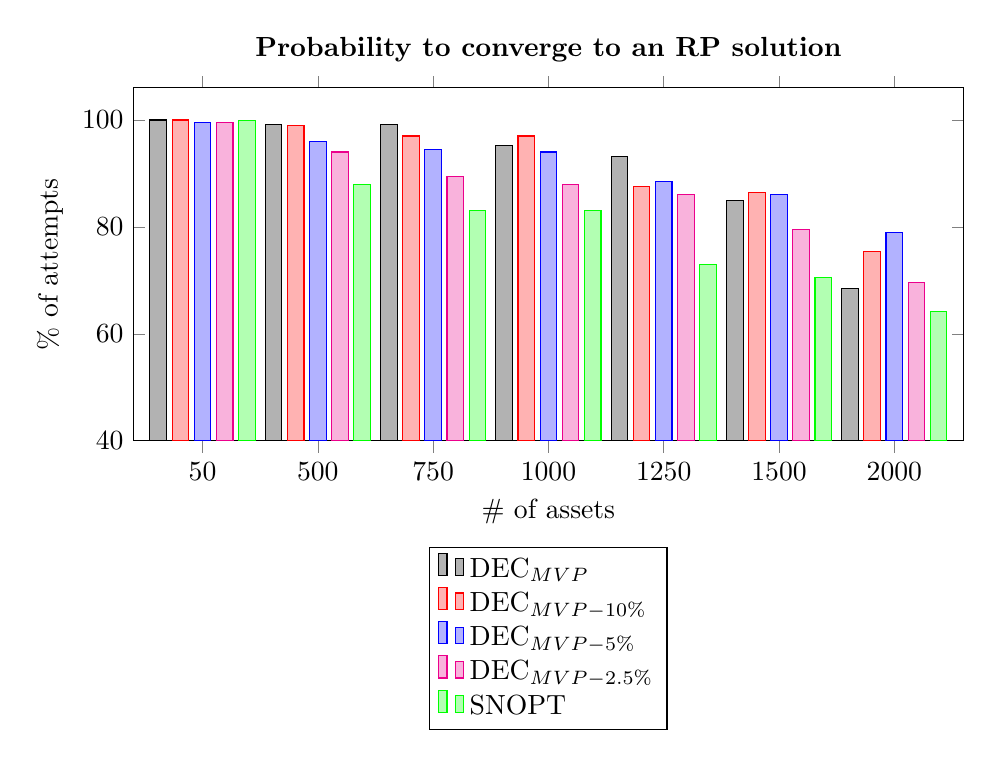
\begin{tikzpicture}
\begin{axis}[%
ybar,
width=1\textwidth,
height=0.5\textwidth,
xlabel={\# of assets},
ylabel={\% of attempts},
ylabel near ticks,
legend pos=south west,
symbolic x coords = {5, 50, 500, 750, 1000, 1250, 1500, 2000},
bar width=6pt,
xtick=data,
ymin=40,
title=\textbf{Probability to converge to an RP solution},
legend cell align=left,
legend style={at={(0.5,-0.3)},anchor=north}
]

 
 \addplot [color=black ,fill=black, fill opacity=0.3] coordinates { %MVP
%(5,100)
(50,100)
(500,99.2)
(750,99.2)
(1000,95.2)
(1250,93.2)
(1500,85.0)
(2000,68.5)
 };
 
\addplot [color=red,fill=red, fill opacity=0.3] coordinates { % 10%
%(5,100)
(50,100)
(500,99.0)     
(750,97.0)    
(1000,97.0)
(1250,87.5)
(1500,86.5)
(2000,75.4)
 };
 
 \addplot [color=blue, fill=blue, fill opacity=0.3] coordinates { % 5%
%(5,100)   
(50,99.5)
(500,96.0)
(750,94.5)
(1000,94)
(1250,88.5)
(1500,86)
(2000,79)
 };
 
 \addplot [color=magenta, fill=magenta, fill opacity=0.3] coordinates { % 2.5%
%(5,100)   
(50,99.5)
(500,94)
(750,89.5)
(1000,88)
(1250,86)
(1500,79.5)
(2000,69.6)
 }; 
 
\addplot [color=green, fill=green, fill opacity=0.3] coordinates { 
%(5,100)         
(50,99.9)
(500,88)
(750,83)
(1000,83)
(1250,73)
(1500,70.5)
(2000,64.2)
 };


\addlegendentry{DEC$_{\text{MVP}}$}
\addlegendentry{DEC$_{\text{MVP-}10\%}$}
\addlegendentry{DEC$_{\text{MVP-}5\%}$}
\addlegendentry{DEC$_{\text{MVP-}2.5\%}$}
\addlegendentry{SNOPT}
\end{axis}
\end{tikzpicture}
}
\caption{Probability to converge to a Risk Parity solution using $x^{0}= [1, 0, .., 0]$ for the decomposition algorithm (with different values of $\lambda$) and SNOPT.}
\label{fig:convergence1}
\end{figure}


\subsubsection{On the choosing of the starting point}
From our experiments, it turns out that the choice of the starting point $x^0$ strongly affects the probability of the algorithms to reach a Risk Parity solution.  In Figure (\ref{fig:sparsity}) we measure the probability to reach a Risk Parity solution varying the sparsity of the initial guess $x^0$, i.e. the percentage of components of $x^0$ fixed to 0. In Figure (\ref{subfig-3:equally}) we use an equally distributed starting point:
\begin{equation}
x^{0} = \left[x^{0}_0, x^{0}_1, .. ,  x^{0}_k, x^{0}_{k+1} .., x^{0}_n \right] = \left[\frac{1}{k}, \frac{1}{k}, .., \frac{1}{k}, 0, .., 0 \right]
\end{equation}
In Figure (\ref{subfig-3:random}) we use a randomly distributed starting point:
\begin{equation}
\begin{aligned}
&a^{0} = \left[r_0, r_1, ..,r_k, 0, .., 0 \right] \qquad \text{where} \quad r_i \sim \mathcal{U}[0,1]\\
&x^0 = \frac{a^{0}}{\mathds{1}^T a^0}
\end{aligned}
\end{equation}
In both case we can observe that a dense starting point leads to a low probability of convergence, especially for larger $n$. In Figure (\ref{subfig-3:equally}) we can notice that when the percentage of sparsity of the starting point exceeds the $40\%$, the probability to converge to an RP solution abruptly increases until it reaches the $100\%$ for each value of $n$ tested. A similar phenomenon is observable in Figure (\ref{subfig-3:random}), but in correspondence of a lower percentage of sparsity of the starting point.

\begin{figure}
\makebox[\textwidth][c]{
\hspace{1em}\subfloat[With equally distributed $x_0$\label{subfig-3:equally}]{%
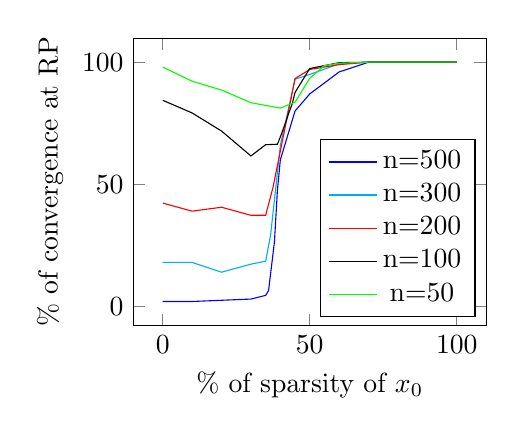
\begin{tikzpicture}
\begin{axis}[%
xlabel={\% of sparsity of $x_0$},
ylabel={\% of convergence at RP},
scaled y ticks=false,
width=0.5\textwidth,
legend pos=south east,
ylabel near ticks
]

\addplot [color=blue,solid,mark=none,mark options={solid}]
  table[row sep=crcr]{%
0 2 \\
10 2 \\
20 2.5 \\
30 3 \\
35 4.5 \\
36 6.5
37 14.5 \\
38 26.5 \\
39 47.5 \\
40 60 \\
45 80\\
50 87 \\
60 96 \\
70 100 \\
80 100 \\
90 100 \\
100 100 \\
};

\addplot [color=cyan,solid,mark=none,mark options={solid}]
  table[row sep=crcr]{%
0 18\\
10 18 \\
20 14 \\
30 17.3 \\
35 18.5 \\
36.67 29.1 \\
38.3 47 \\
40 66 \\
45 93 \\
50 95 \\
60 99.3 \\
70 100 \\
80 100 \\
90 100 \\
100 100\\
};

\addplot [color=red,solid,mark=none,mark options={solid}]
  table[row sep=crcr]{%
0 42.3 \\
10 39 \\
20 40.6 \\
30 37.3 \\
35 37.3 \\
37.5 48.7 \\
38.5 54.7 \\
40 63.6 \\
45 93.3 \\
50 97 \\
60 99 \\
70 100 \\
80 100 \\
90 100 \\
100 100\\
};

\addplot [color=black,solid,mark=none,mark options={solid}]
  table[row sep=crcr]{%
0 84.4 \\
10 79.2 \\
20 71.8 \\
30 61.6 \\
35 66.2 \\
39 66.4 \\
40 69.4 \\
42 76 \\
43 79.6 \\
44 82.8\\
45 87.6 \\
50 97.4 \\
60 99.8 \\
70 100 \\
80 100 \\
90 100 \\
100 100\\
};

\addplot [color=green,solid,mark=none,mark options={solid}]
  table[row sep=crcr]{%
0 98 \\
10 92.2 \\
20 88.6\\
30 83.4 \\
40 81.2 \\
45 83.6 \\
50 93.4 \\
55 98.6 \\
60 99.6 \\
70 100 \\
80 100 \\
90 100 \\
100 100 \\
};
\addlegendentry{n=500}
\addlegendentry{n=300}
\addlegendentry{n=200}
\addlegendentry{n=100}
\addlegendentry{n=50}
\end{axis}
\end{tikzpicture}
}
\hspace{1em}\subfloat[With random $x_0$\label{subfig-3:random}]{%
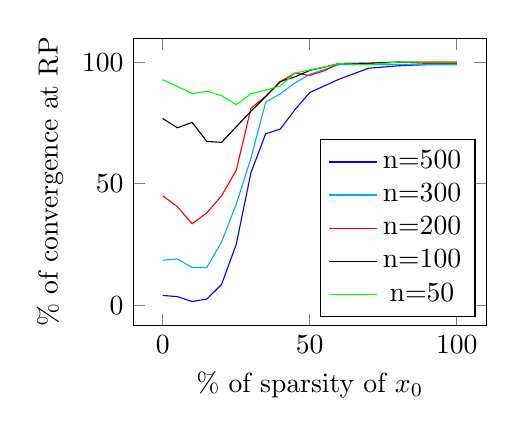
\begin{tikzpicture}
\begin{axis}[%
width=0.5\textwidth,
xlabel={\% of sparsity of $x_0$},
ylabel={\% of convergence at RP},
legend pos=south east,
ylabel near ticks
]

\addplot [color=blue,solid,mark=none,mark options={solid}]
  table[row sep=crcr]{%
0  4.0 \\
5  3.5 \\
10 1.5 \\
15 2.5 \\
20 8.5 \\
25 25.0 \\
30 54.5 \\
35 70.5 \\
40 72.5 \\
45 80.5 \\
50 87.5 \\
60 93 \\
70 97.5 \\
80 98.5 \\
90 99.0 \\
100 99.0 \\
};

\addplot [color=cyan,solid,mark=none,mark options={solid}]
  table[row sep=crcr]{%
0 18.5 \\
5 19.0 \\
10 15.5 \\
15 15.5 \\
20 26.0 \\
25 41.5 \\
30 60.5 \\
35 83.5 \\
40 87.0 \\
45 91.5 \\
50 95.0 \\
60 99.0 \\
90 99.0 \\
100 99.0 \\
};

\addplot [color=red,solid,mark=none,mark options={solid}]
  table[row sep=crcr]{%
0 45 \\
5 40.5 \\
10 33.5 \\
15 38.0 \\
20 45.0 \\
25 55.5 \\
30 81.0 \\
35 86.0 \\
40 92.0 \\
45 95.5 \\
50 94.5 \\
55 96.5 \\
60 99.5 \\
70 99.5 \\
80 100 \\
90 99.5 \\
100 99.5 \\
};

\addplot [color=black,solid,mark=none,mark options={solid}]
  table[row sep=crcr]{%
0 76.8 \\
5 73 \\
10 75.2 \\
15 67.4 \\
20 67 \\
25 73.4 \\
30 79.8 \\
35 85.8 \\
40 92 \\
45 94 \\
50 96.6 \\
55 98 \\
60 99.4 \\
70 99.6 \\
80 100 \\
90 100 \\
100 100 \\
};

\addplot [color=green,solid,mark=none,mark options={solid}]
  table[row sep=crcr]{%
0 92.8\\
5 90 \\
10 87.0 \\
15 88.0 \\
20 86.2\\
25 82.5 \\
30 87.0 \\
35 88.5 \\
40 90.2 \\
45 95.5 \\
50 96.8 \\
55 98.0 \\
60 99.4 \\
70 99.0 \\
80 100 \\
90 100 \\
100 100\\
};


\addlegendentry{n=500}
\addlegendentry{n=300}
\addlegendentry{n=200}
\addlegendentry{n=100}
\addlegendentry{n=50}
\end{axis}
\end{tikzpicture}
}
}
\caption{Percentage of computations of DEC$_{\text{MVP}}$ that find an RP solution, varying the sparsity of the initial guess $x^0$, for different number of assets $n$}
\label{fig:sparsity}
\end{figure}

\subsection{General box constraints}
In this section we use different combinations for the box constraints $l$ and $u$ and we compare the values assumed by the objective function in the critical point reached by the different algorithms. In these tests we take:
\begin{equation}\label{eq:startxx}
x_i^0 = \frac{1}{n} \quad \forall i 
\end{equation}

\subsubsection{Execution Time}
In Figure (\ref{fig:ultima1}) we compare the average execution time and the average number of iterations performed by the decomposition algorithm (with different values of $\lambda$) against SNOPT using the starting point defined in (\ref{eq:startxx}) and 
\begin{equation}\label{eq:generalbox}
l_i = \frac{1}{2n}  \qquad u_i = \frac{2}{n}  \quad \forall i
\end{equation} 
The $\epsilon$ in the stop criterion (\ref{eq:stop}) is set to $10^{-10}$.\\ The results reported in Figure (\ref{subfig-1:time1}) shows that SNOPT is the fastest algorithm to converge when we use this kind of bounds. For $n=2000$, SNOPT takes $2.68$ seconds to converge, while the fastest decomposition algorithm (DEC$_{\text{MVP-}2.5\%}$) takes $6.64$ seconds.\\
Comparing Figure (\ref{subfig-2:iterations1}) with Figure (\ref{subfig-2:iterations2}) and Figure (\ref{subfig-2:iterations3}) we can deduce that all the decomposition algorithms tested takes less iterations to converge to a critical point when initialized with the equally weighted starting point (\ref{eq:startxx}).
\begin{figure}
\makebox[\textwidth][c]{
\subfloat[Comparison of average execution time\label{subfig-1:time1}]{
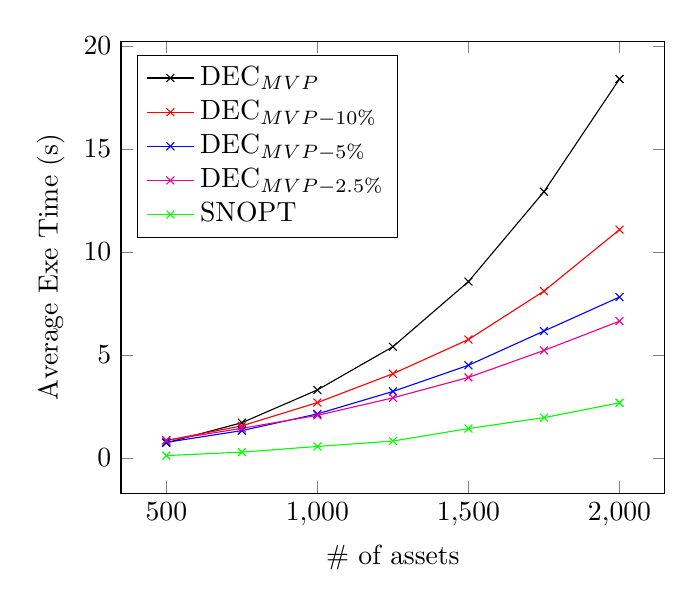
\begin{tikzpicture}
\begin{axis}[%
width=0.7\textwidth,
xlabel={\# of assets},
ylabel={Average Exe Time (s)},
scaled y ticks=false,
legend pos=north west,
legend cell align=left
]

\addplot [color=black,solid,mark=x,mark options={solid}]
  table[row sep=crcr]{%
%100	.105\\
%200	.214\\
%300	.340\\
500	.737	\\
750	1.713		\\
1000 3.303 \\
1250 5.400 \\
1500 8.56\\
1750 12.92\\
2000 18.39\\
};

\addplot [color=red,solid,mark=x,mark options={solid}]
  table[row sep=crcr]{%10
%100 .146\\
%250 .341\\
500 .853\\
750 1.56\\
1000 2.69 \\
1250 4.09\\
1500 5.75\\
1750 8.10\\
2000 11.08\\
};

\addplot [color=blue,solid,mark=x,mark options={solid}]
  table[row sep=crcr]{%5
%100 .190\\
%250 .355\\
500 .759 \\
750 1.33 \\
1000 2.14 \\
1250 3.23\\
1500 4.50 \\
1750 6.16 \\
2000 7.81 \\
};

\addplot [color=magenta,solid,mark=x,mark options={solid}]
  table[row sep=crcr]{%2.5
%100 .299\\
%250 .468\\
500  .854\\
750  1.44\\
1000 2.07 \\
1250 2.92 \\
1500 3.91 \\
1750 5.22 \\
2000 6.64\\
};
\addplot [color=green,solid,mark=x,mark options={solid}]
  table[row sep=crcr]{%
%100	.005	\\
%200	.014	\\
%300	.035	    \\
500	.118	    \\
750	 .286  \\
1000 0.561	\\
1250 0.824	\\
1500 1.43 \\
1750 1.96 \\
2000 2.68\\
};

\addlegendentry{DEC$_{\text{MVP}}$}
\addlegendentry{DEC$_{\text{MVP-}10\%}$}
\addlegendentry{DEC$_{\text{MVP-}5\%}$}
\addlegendentry{DEC$_{\text{MVP-}2.5\%}$}
\addlegendentry{SNOPT}
\end{axis}

\end{tikzpicture}
}
}
\hfill
\hspace{1em}\subfloat[Comparison of average iterations\label{subfig-2:iterations1}]{%
\makebox[\textwidth][c]{
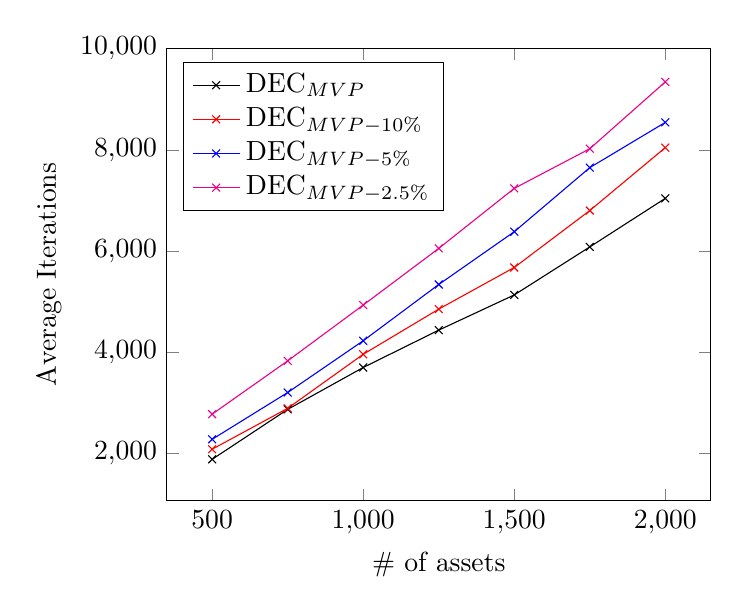
\begin{tikzpicture}

\begin{axis}[%
width=0.7\textwidth,
xlabel={\# of assets},
ylabel={Average Iterations},
ymax=10000,
scaled y ticks=false,
legend pos=north west,
legend cell align=left
]

\addplot [color=black,solid,mark=x,mark options={solid}]
  table[row sep=crcr]{%MVP
%100	445 \\
%200	819 \\
%300	1176 \\
500	1888\\
750	2874 \\
1000	 3701\\
1250	 4439\\
1500 5134\\
1750 6082\\
2000 7041\\
};

\addplot [color=red,solid,mark=x,mark options={solid}]
  table[row sep=crcr]{%10
%100 607\\
%250 1134\\
500 2087\\ 
750 2895 \\
1000 3962 \\
1250 4854 \\
1500 5676 \\
1750 6800 \\
2000 8043\\
};

\addplot [color=blue,solid,mark=x,mark options={solid}]
  table[row sep=crcr]{%5
%100 841\\
%250 1349\\
500 2283   \\
750 3207 \\
1000 4229  \\
1250 5340 \\
1500 6382 \\
1750 7648\\
2000 8541\\
};

\addplot [color=magenta,solid,mark=x,mark options={solid}]
  table[row sep=crcr]{%2.5
%100 1346\\
%250 1857\\
500 2780 \\
750 3832\\
1000 4934  \\
1250 6053\\
1500 7238\\
1750 8021\\
2000 9341\\
};

\addlegendentry{DEC$_{\text{MVP}}$}
\addlegendentry{DEC$_{\text{MVP-}10\%}$}
\addlegendentry{DEC$_{\text{MVP-}5\%}$}
\addlegendentry{DEC$_{\text{MVP-}2.5\%}$}
\end{axis}

\end{tikzpicture}
}
}
\caption{Comparison of performances using $\epsilon = 10^{-10}$ in (\ref{eq:stop}) with box constraints defined in (\ref{eq:generalbox})}
\label{fig:ultima1}
\end{figure}

\subsubsection{Quality of the solutions produced}
We denote with $x_{D}$ the solution produced by DEC$_{\text{MVP}}$ and with $x_{S}$ the solution produced by SNOPT. In Figure (\ref{fig:box}), we compare the value of $f(x_{D})$ with $f(x_{S})$ when the two algorithms converges at two different critical points ($x_D \neq x_S$) using different combinations of box constraints.\\ Figure (\ref{fig:box}) points out that DEC$_{\text{MVP}}$ converges to points with a better value of the objective function than SNOPT for three combinations of bounds out of four. For example, using
\begin{equation*}
l_i = \frac{1}{2n}, \quad u_i = \frac{2}{n} \quad \forall i
\end{equation*}
and $n=500$, DEC$_{\text{MVP}}$ finds better solutions than SNOPT in the $40\%$ of the total attempts. The only case in which SNOPT finds better solutions than DEC$_{\text{MVP}}$ is when we use
\begin{equation*}
l_i = -1, \quad u_i = 1 \quad \forall i
\end{equation*} 

\begin{figure}
\makebox[\textwidth][c]{

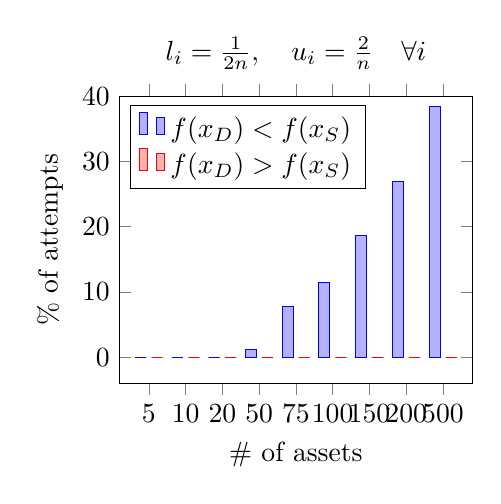
\begin{tikzpicture}
\begin{axis}[%
ybar,
xlabel={\# of assets},
ylabel={\% of attempts},
ylabel near ticks,
legend pos=north west,
symbolic x coords = {5,10,20,50,75,100,150,200,500},
bar width=4pt,
xtick=data,
ymax=40,
width=.5\textwidth,
title={$l_i = \frac{1}{2n}, \quad u_i = \frac{2}{n} \quad \forall i$},
]
\addplot coordinates { 
(5,0)         
(10,0)
(20,0)
(50,1.2)
(75,7.8)
(100,11.5)
(150,18.7)
(200,26.9)
(500,38.4)
 };
 
 \addplot coordinates { 
(5,0)         
(10,0)
(20,0)
(50,0)
(75,0)
(100,0)
(150,0)
(200,0)
(500,0)
 };

\addlegendentry{$f(x_{D}) < f(x_{S})$}
\addlegendentry{$f(x_{D}) > f(x_{S})$}
\end{axis}
\end{tikzpicture}


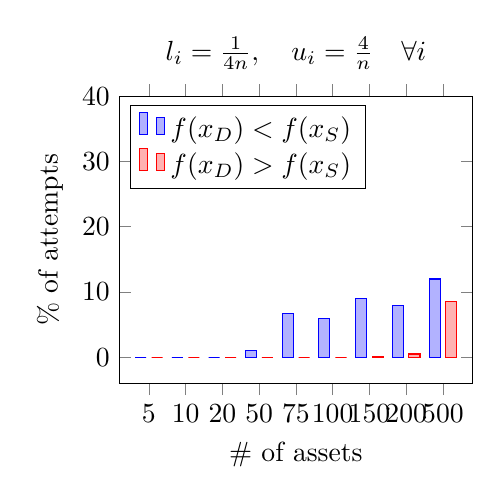
\begin{tikzpicture}
\begin{axis}[%
ybar,
xlabel={\# of assets},
ylabel={\% of attempts},
ylabel near ticks,
legend pos=north west,
symbolic x coords = {5,10,20,50,75,100,150,200,500},
bar width=4pt,
xtick=data,
ymax=40,
width=.5\textwidth,
title={$l_i = \frac{1}{4n}, \quad u_i = \frac{4}{n} \quad \forall i$}
]
\addplot coordinates { 
(5,0)         
(10,0)
(20,0)
(50,1.0)
(75,6.7)
(100,6.0)
(150,9.0)
(200,7.9)
(500,12.0)
 };
 
 \addplot coordinates { 
(5,0)         
(10,0)
(20,0)
(50,0)
(75,0)
(100,0)
(150,0.1)
(200,0.5)
(500,8.6)
 };

\addlegendentry{$f(x_{D}) < f(x_{S})$}
\addlegendentry{$f(x_{D}) > f(x_{S})$}
\end{axis}
\end{tikzpicture}
}

\makebox[\textwidth][c]{
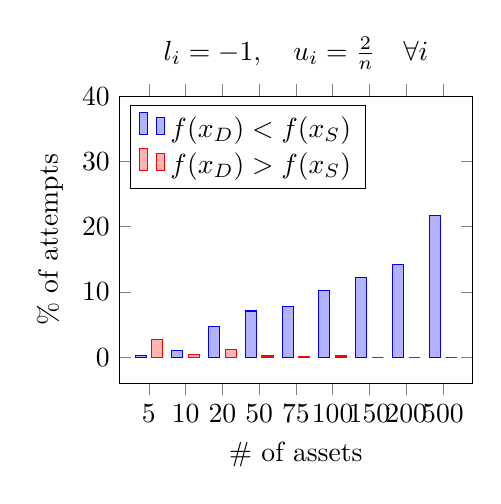
\begin{tikzpicture}
\begin{axis}[%
ybar,
xlabel={\# of assets},
ylabel={\% of attempts},
ylabel near ticks,
legend pos=north west,
symbolic x coords = {5,10,20,50,75,100,150,200,500},
bar width=4pt,
xtick=data,
ymax=40,
width=.5\textwidth,
title={$l_i = -1, \quad u_i = \frac{2}{n} \quad \forall i$}
]
\addplot coordinates { 
(5,0.3)         
(10,1.0)
(20,4.7)
(50,7.1)
(75,7.8)
(100,10.2)
(150,12.2)
(200,14.2)
(500,21.7)
 };
 
 \addplot coordinates { 
(5,2.7)         
(10,0.4)
(20,1.2)
(50,0.2)
(75,0.1)
(100,0.2)
(150,0)
(200,0)
(500,0)
 };

\addlegendentry{$f(x_{D}) < f(x_{S})$}
\addlegendentry{$f(x_{D}) > f(x_{S})$}
\end{axis}
\end{tikzpicture}
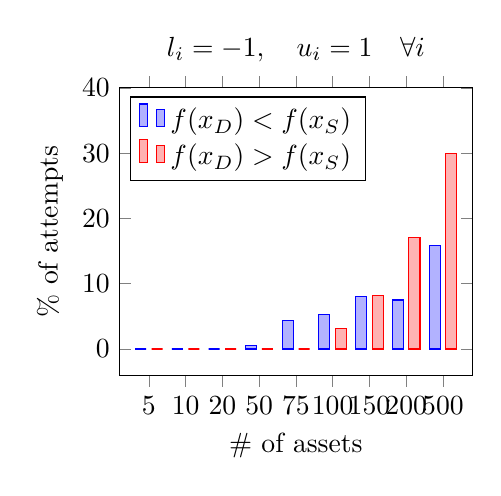
\begin{tikzpicture}
\begin{axis}[%
ybar,
xlabel={\# of assets},
ylabel={\% of attempts},
ylabel near ticks,
legend pos=north west,
symbolic x coords = {5,10,20,50,75,100,150,200,500},
bar width=4pt,
xtick=data,
ymax=40,
width=.5\textwidth,
title={$l_i = -1, \quad u_i = 1 \quad \forall i$}
]
\addplot coordinates { 
(5,0)         
(10,0)
(20,0)
(50,0.6)
(75,4.4)
(100,5.3)
(150,8.0)
(200,7.5)
(500,15.9)
 };
 
 \addplot coordinates { 
(5,0)         
(10,0)
(20,0)
(50,0)
(75,0)
(100,3.2)
(150,8.2)
(200,17.1)
(500,30)
 };

\addlegendentry{$f(x_{D}) < f(x_{S})$}
\addlegendentry{$f(x_{D}) > f(x_{S})$}
\end{axis}
\end{tikzpicture}
}
\caption{Comparison of objective function values for $x_{D}$ and $x_{S}$ with different box constraints. For each $n$ we perform $1000$ experiments for both the algorithms.}
\label{fig:box}
\end{figure}

